\documentclass[12pt,a4paper]{article}
\usepackage{parskip}
\usepackage{graphicx}
\usepackage{eurosym}
\usepackage{ngerman}
\usepackage[utf8x]{inputenc}
\usepackage[T1]{fontenc}
\usepackage{hyperref}
\usepackage{fancyhdr}
\usepackage[left=2cm,right=2cm,top=1.5cm,bottom=1.5cm,includeheadfoot,a4paper]{geometry}
\usepackage{wrapfig}
\usepackage{fontspec}
\usepackage{longtable}
\usepackage{booktabs}
\setmainfont{Ubuntu}
\setmonofont{Ubuntu Mono}

\setlength{\parindent}{0pt}%Wenn Absatzabstand, dann Einzug unnötig

\pagestyle{fancy}


\fancyhead{}
\fancyfoot{}
%\fancyfoot[L]{rev: \GITAbrHash}
\fancyfoot[C]{\thepage}
\renewcommand{\headrulewidth}{0pt}
\renewcommand{\footrulewidth}{0pt}

\include{vc}

\providecommand{\tightlist}{%
  \setlength{\itemsep}{0pt}\setlength{\parskip}{0pt}}

\begin{document}
\begin{titlepage}
	\centering
	\includegraphics[width=0.5\textwidth]{pics/logo.eps}\par\vspace{1cm}
  {\scshape\Huge Finanzbericht 2017 \par}
	\vfill

% Bottom of the page
	{\scshape\large \today\par}
	{\scshape\large vspace.one e.V. \par}
	{\scshape\large Ludwig-Weißer-Str. 3 \par}
	{\scshape\large 78112 St.Georgen \par}
	{\scshape\large rev: \GITAbrHash \par}
	\vspace{1cm}
\end{titlepage}

\section{Gewinne und Verluste 2017}

\begin{tabular}{ l|r }
  Erträge:Mitgliedsbeiträge & 1.292,00 EUR \\
  Erträge:Zweckgebundene Spende & 100,00 EUR \\
  Erträge:Wirtschaftlicher Geschäftsbetrieb & 165,00 EUR \\
  \hline
  Aufwendungen:Einrichtung & 129,78 EUR \\
  Aufwendungen:Equipment & 806,70 EUR \\
  Aufwendungen:Kontoführung & 36,70 EUR \\
  Aufwendungen:Projekte & 67,83 EUR \\
  Aufwendungen:Verbrauch & 253,07 EUR \\
  Aufwendungen:Werbung & 161,70 EUR \\
  \hline
  Summe & \textbf{101,22} EUR \\

\end{tabular}

\section{Kontostand}
\begin{tabular}{ l|r }
Bankkonto & \textbf{576,89} EUR \\
Offene Forderungen & \textbf{133,00} EUR \\
Barkasse & \textbf{81.62} EUR \\

\end{tabular}

\section{Konten}
\subsection{Erträge:Mitgliedsbeiträge}
Hier fließen die Mitgliedbeiträge rein. Außerdem eventuelle Gebühren für Retouren der Lastschriften.

\subsection{Erträge:Zweckgebundene Spenden}
Enthält dieses Jahr nur eine Spende der Volksbank. Die Spende war zur Finanzierung des 3D-Druckers gedacht und wurde auch so verwendet.

\subsection{Erträge:Wirtschaftlicher Geschäftsbetrieb}
Im vspace.one stellen wir Getränke für einen Umkostenbeitrag von 1 Euro zur Verfügung. Da bleibt immer ein bisschen was hängen, weil das nicht ganz der Einkaufspreis ist. Einnahmen hieraus sind hier zu finden.

\subsection{Aufwendungen:Einrichtungen}
Hier sind Gegenstände der Einrichtung, wie Arbeitsplatten, Projektboxen usw. enthalten.

\subsection{Aufwendungen:Equipment}
Im wesentlichen war das dieses Jahr ein 3D-Drucker für 600 Euro. Außerdem Feinstaubmasken für die Fräse, Schutzbrillen und diverses anderes nützliches Equipment.

\subsection{Aufwendungen:Kontoführung}
Hier fließen die Kosten für das Vereinskonto bei der Volksbank rein.

\subsection{Aufwendungen:Projekte}
Projektkosten für einzelne ausgewählte Projekte von Mitgliedern. Dieses Jahr war es nur ein Projekt damit beschäftigt das Schließsystem des vspace.one zu verbessern. Das Projekt läuft noch.

\subsection{Aufwendungen:Verbrauch}
Hier sind verschiedene Verbrauchsgegenstände, wie Schleifpapier, Sprühkleber sowie Gehörschutz zu finden.

\subsection{Aufwendungen:Werbung}
Der Bereich Werbung umfasst alles was Kosten für Aufkleber, Plakate sowie die Webseite ist.

\section{Diagramme}

\begin{figure}
  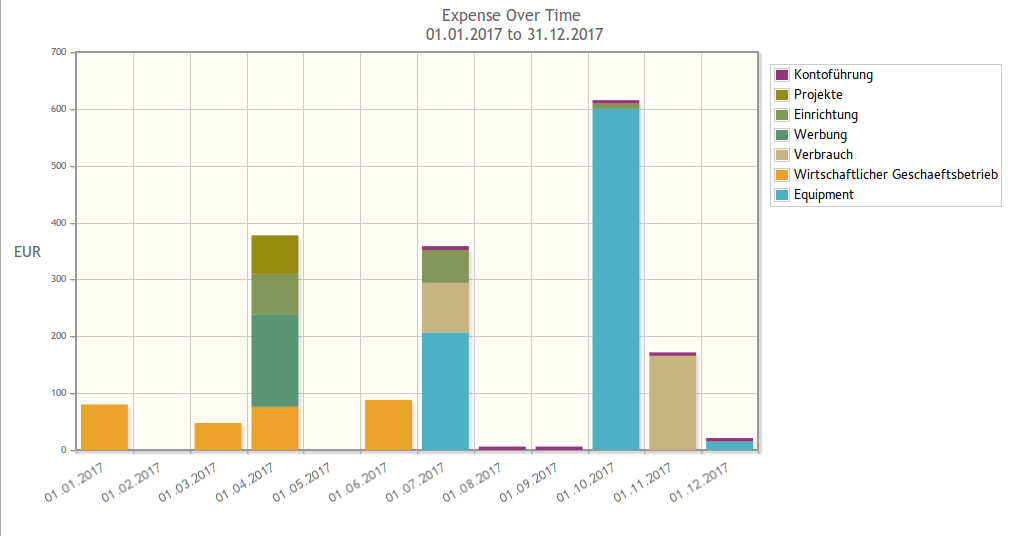
\includegraphics[width=\linewidth]{pics/expense_2017.png}
\end{figure}



\end{document}
